\documentclass[tikz, convert={convertexe=magick}, png]{standalone}

\usepackage{yquant, braket}
\yquantset{register/default name=$\ket{\reg_{\idx}}$}

\begin{document}
   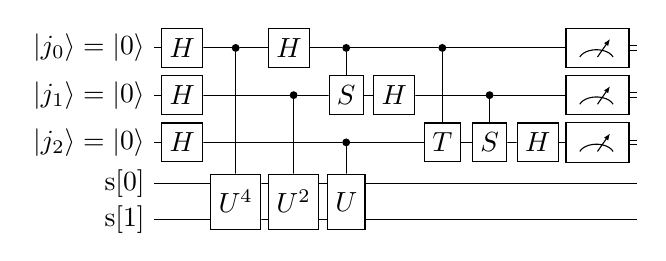
\begin{tikzpicture}
      \begin{yquant}
         qubit {$\ket{j_{\idx}} = \ket0$} j[3];
         qubit s[2];
         
         h j;
         box {$U^4$} (s) | j[0];
         box {$U^2$} (s) | j[1];
         box {$U$} (s) | j[2];
         h j[0];
         box {$S$} j[1] | j[0];
         h j[1];
         box {$T$} j[2] | j[0];
         box {$S$} j[2] | j[1];
         h j[2];
         measure j;
      \end{yquant}
   \end{tikzpicture}
\end{document}